\justy{Poniżej zaprezentowano wstępne makiety ekranów jakie będą używane w aplikacji mobilnej, do obsługi dodawania użytkownika do kolejki, dzwonienia, odbierania połączeń, rozmowy i kończenia rozmowy. Wszystkie ekrany są jedynie koncepcją interfejsu i nie należy traktować ich jako produktu końcowego.}

 \justy{Aktualizacja z finalnego produktu: poniższe makiety ekranów zostały zmienione ze względu na przeniesienie aplikacji klienckiej na urządzenia z systemem Windows, wygląd makiet nieznacznie odbiega od ekranów przedstawionych już w gotowym produkcie.}
\hfil


\begin{figure}[H]
	\centering
	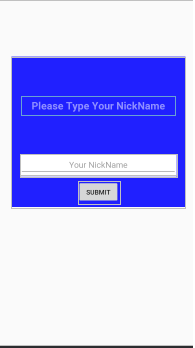
\includegraphics[width=8cm]{images/5.png}
	\caption{\centering Pierwszy ekran z prośbą o podanie pseudonimu użytkownika.}
	\hfill 
\end{figure} 
\begin{figure}[H]
	\centering
	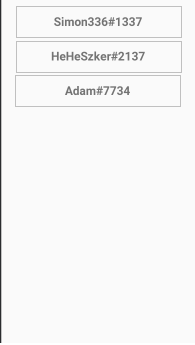
\includegraphics[width=8cm]{images/1.png}
	\caption{\centering Ekran z widoczną ''poczekalnią'', w której znajduje się trzech użytkowników.}
	\hfill 
\end{figure} 
\begin{figure}[H]
	\centering
	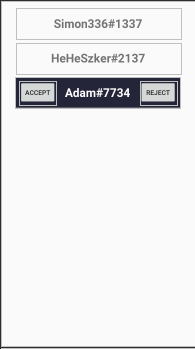
\includegraphics[width=8cm]{images/2.png}
	\caption{\centering Informacja o nadchodzącym połączenia od użytkownika Adam.}
	\hfill 
\end{figure} 
\begin{figure}[H]
	\centering
	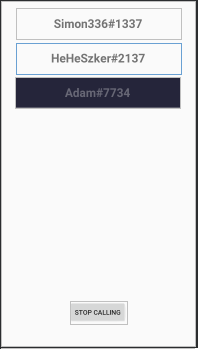
\includegraphics[width=8cm]{images/3.png}
	\caption{\centering Próba połączenia się z użytkownikiem Adam.}
	\hfill 
\end{figure} 
\begin{figure}[H]
	\centering
	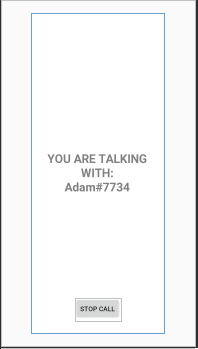
\includegraphics[width=8cm]{images/4.png}
	\caption{\centering Rozmowa z użytkownikiem Adam.}
	\hfill 
\end{figure}
\hfill